%% fcup-thesis.tex -- document template for PhD theses at FCUP
%%
%% Copyright (c) 2015 João Faria <joao.faria@astro.up.pt>
%%
%% This work may be distributed and/or modified under the conditions of
%% the LaTeX Project Public License, either version 1.3c of this license
%% or (at your option) any later version.
%% The latest version of this license is in
%%     http://www.latex-project.org/lppl.txt
%% and version 1.3c or later is part of all distributions of LaTeX
%% version 2005/12/01 or later.
%%
%% This work has the LPPL maintenance status "maintained".
%%
%% The Current Maintainer of this work is
%% João Faria <joao.faria@astro.up.pt>.
%%
%% This work consists of the files listed in the accompanying README.

%% SUMMARY OF FEATURES:
%%
%% All environments, commands, and options provided by the `ut-thesis'
%% class will be described below, at the point where they should appear
%% in the document.  See the file `ut-thesis.cls' for more details.
%%
%% To explicitly set the pagestyle of any blank page inserted with
%% \cleardoublepage, use one of \clearemptydoublepage,
%% \clearplaindoublepage, \clearthesisdoublepage, or
%% \clearstandarddoublepage (to use the style currently in effect).
%%
%% For single-spaced quotes or quotations, use the `longquote' and
%% `longquotation' environments.


%%%%%%%%%%%%         PREAMBLE         %%%%%%%%%%%%

%%  - Default settings format a final copy (single-sided, normal
%%    margins, one-and-a-half-spaced with single-spaced notes).
%%  - For a rough copy (double-sided, normal margins, double-spaced,
%%    with the word "DRAFT" printed at each corner of every page), use
%%    the `draft' option.
%%  - The default global line spacing can be changed with one of the
%%    options `singlespaced', `onehalfspaced', or `doublespaced'.
%%  - Footnotes and marginal notes are all single-spaced by default, but
%%    can be made to have the same spacing as the rest of the document
%%    by using the option `standardspacednotes'.
%%  - The size of the margins can be changed with one of the options:
%%     . `narrowmargins' (1 1/4" left, 3/4" others),
%%     . `normalmargins' (1 1/4" left, 1" others),
%%     . `widemargins' (1 1/4" all),
%%     . `extrawidemargins' (1 1/2" all).
%%  - The pagestyle of "cleared" pages (empty pages inserted in
%%    two-sided documents to put the next page on the right-hand side)
%%    can be set with one of the options `cleardoublepagestyleempty',
%%    `cleardoublepagestyleplain', or `cleardoublepagestylestandard'.
%%  - Any other standard option for the `report' document arclass can be
%%    used to override the default or draft settings (such as `10pt',
%%    `11pt', `12pt'), and standard LaTeX packages can be used to
%%    further customize the layout and/or formatting of the document.

%% *** Add any desired options. ***
%PDF
%\documentclass[a4paper,narrowmargins,12pt,oneside,draft,onehalfspaced,singlespacednotes]{fcup-thesis}
%\documentclass[a4paper,narrowmargins,12pt,oneside,onehalfspaced,singlespacednotes]{fcup-thesis}
%Print
%\documentclass[draft,a4paper,narrowmargins,12pt,twoside,openright,onehalfspaced,singlespacednotes]{fcup-thesis}
\documentclass[a4paper,narrowmargins,12pt,twoside,openright,onehalfspaced,singlespacednotes]{fcup-thesis}

%% *** Add \usepackage declarations here. ***
%% The standard packages `geometry' and `setspace' are already loaded by
%% `ut-thesis' -- see their documentation for details of the features
%% they provide.  In particular, you may use the \geometry command here
%% to adjust the margins if none of the ut-thesis options are suitable
%% (see the `geometry' package for details).  You may also use the
%% \setstretch command to set the line spacing to a value other than
%% single, one-and-a-half, or double spaced (see the `setspace' package
%% for details).
% Overfull statements
\pretolerance=150
\setlength{\emergencystretch}{3em}
% Overfull end
\usepackage[english]{babel}
\usepackage{lipsum}
\usepackage[utf8]{inputenc}


%%% Additional useful packages
%%% ----------------------------------------------------------------
\usepackage{array}
\usepackage{amsmath}  
\usepackage{amssymb}
\usepackage{amsfonts}
\DeclareFontFamily{OT1}{pzc}{}
\DeclareFontShape{OT1}{pzc}{m}{it}{<-> s * [0.900] pzcmi7t}{}
\DeclareMathAlphabet{\mathpzc}{OT1}{pzc}{m}{it}
\usepackage{amsthm}      
\usepackage[ruled,algochapter]{algorithm2e}
\usepackage{algorithmic}
\usepackage{bm}
\usepackage[mathscr]{euscript}
\usepackage{graphicx}       
\usepackage{psfrag}         
\usepackage{fancyvrb}    
\usepackage{float}
\usepackage{ltablex}
\usepackage[square,sort,comma,numbers]{natbib}        
\usepackage{bbding}         
\usepackage{dcolumn}        
\usepackage{booktabs} 
\usepackage{multirow}
\usepackage{paralist}     
\usepackage{ifdraft}  
\usepackage{indentfirst}    
\usepackage[nottoc,notlof,notlot]{tocbibind}
\usepackage{url}
\usepackage{tabularx}
\usepackage{subcaption}
\usepackage[unicode]{hyperref}
\usepackage{xcolor}

\hypersetup{pdftitle=LiDAR obstacle detection and avoidance, 
            pdfauthor=Alojz Gomola,
            colorlinks=false,
            urlcolor=blue,
            pdfstartview=FitH,
            pdfpagemode=UseOutlines,
            pdfnewwindow,
            breaklinks
          }
\usepackage{array}
\newcolumntype{L}[1]{>{\raggedright\let\newline\\\arraybackslash\hspace{0pt}}m{#1}}
\newcolumntype{C}[1]{>{\centering\let\newline\\\arraybackslash\hspace{0pt}}m{#1}}
\newcolumntype{R}[1]{>{\raggedleft\let\newline\\\arraybackslash\hspace{0pt}}m{#1}}         
\newcolumntype{B}{X}
\newcolumntype{S}[1]{>{\hsize=#1\textwidth}X}

\newcommand{\FIGDIR}{./Pics}    %%% directory containing figures
\newcommand{\twolinecellr}[2][r]{%
  \begin{tabular}[#1]{@{}r@{}}#2\end{tabular}}
\newcommand{\secState}[1]{
	\ifdraft{(#1) }{}
}
\theoremstyle{plain}
\newtheorem{theorem}{Theorem}
\newtheorem{lemma}[theorem]{Lemma}
\newtheorem{proposition}[theorem]{Proposition}

\theoremstyle{plain}
\newtheorem{definition}{Definition}
\newtheorem{problem}{Problem}
\newtheorem{example}{Example}
\newtheorem{assumption}{Assumption}

\theoremstyle{remark}
\newtheorem*{corollary}{Corollary}
\newtheorem*{note}{Note}




\newenvironment{dokaz}{
  \par\medskip\noindent
  \textit{Proof}.
}{
\newline
\rightline{\SquareCastShadowBottomRight}
}

\newenvironment{constraints}[1]{
  \par\medskip\noindent
  \textit{Constraints #1} \\
}{
\newline
\rightline{\SquareCastShadowBottomRight}
}


%\bibliographystyle{plainnat}     %% Author (year) style
\bibliographystyle{unsrt}        %% [number] style
\setcitestyle{square}

% Section  3.7 Challenge list
\newif\ifproblemchallenge   %# Build block for problem challenges
\problemchallengetrue       %# Show comments

\newcommand{\R}{\mathbb{R}}
\newcommand{\N}{\mathbb{N}}

\DeclareMathOperator{\pr}{\textsf{P}}
\DeclareMathOperator{\E}{\textsf{E}\,}
\DeclareMathOperator{\var}{\textrm{var}}
\DeclareMathOperator{\sd}{\textrm{sd}}


\newcommand{\T}[1]{#1^\top}        

\newcommand{\goto}{\rightarrow}
\newcommand{\gotop}{\stackrel{P}{\longrightarrow}}
\newcommand{\maon}[1]{o(n^{#1})}
\newcommand{\abs}[1]{\left|{#1}\right|}
\newcommand{\dint}{\int_0^\tau\!\!\int_0^\tau}
\newcommand{\isqr}[1]{\frac{1}{\sqrt{#1}}}
\newcommand{\norm}[1]{\left\lVert#1\right\rVert}


\newcommand{\pulrad}[1]{\raisebox{1.5ex}[0pt]{#1}}
\newcommand{\mc}[1]{\multicolumn{1}{c}{#1}}
\newcommand{\TBD}[1]{\color{red}\emph{--TBD:}#1\color{black}}

%%%%%%%%%%%%%%%%%%%%%%%%%%%%%%%%%%%%%%%%%%%%%%%%%%%%%%%%%%%%%%%%%%%%%%%%
%%                                                                    %%
%%                   ***   I M P O R T A N T   ***                    %%
%%                                                                    %%
%%  Fill in the following fields with the required information:       %%
%%   - \degree{...}       name of the degree obtained                 %%
%%   - \department{...}   name of the graduate department             %%
%%   - \gradyear{...}     year of graduation                          %%
%%   - \author{...}       name of the author                          %%
%%   - \title{...}        title of the thesis                         %%
%%%%%%%%%%%%%%%%%%%%%%%%%%%%%%%%%%%%%%%%%%%%%%%%%%%%%%%%%%%%%%%%%%%%%%%%

%% *** Change this example to appropriate values. ***
\degree{Doctor of Philosophy}
\department{Departamento de Matem\'{a}tica}
\gradyear{2019}
\author{Alojz Gomola}
\title{Obstacle Avoidance Framework based on Reach Sets}

%% *** NOTE ***
%% Put here all other formatting commands that belong in the preamble.
%% In particular, you should put all of your \newcommand's,
%% \newenvironment's, \newtheorem's, etc. (in other words, all the
%% global definitions that you will need throughout your thesis) in a
%% separate file and use "\input{filename}" to input it here.


%% *** Adjust the following settings as desired. ***

%% List only down to subsections in the table of contents;
%% 0=chapter, 1=section, 2=subsection, 3=subsubsection, etc.
\setcounter{tocdepth}{3}

%% Make each page fill up the entire page.
\flushbottom


%%%%%%%%%%%%      MAIN  DOCUMENT      %%%%%%%%%%%%

\begin{document}


%%%%%%%%%%%%%%%%%%%%%%%%%%%%%%%%%%%%%%%%%%%%%%%%%%%%%%%%%%%%%%%%%%%%%%%%
%%  Put your Chapters here; the easiest way to do this is to keep     %%
%%  each chapter in a separate file and `\include' all the files.     %%
%%  Each chapter file should start with "\chapter{ChapterName}".      %%
%%  Note that using `\include' instead of `\input' will make each     %%
%%  chapter start on a new page, and allow you to format only parts   %%
%%  of your thesis at a time by using `\includeonly'.                 %%
%%%%%%%%%%%%%%%%%%%%%%%%%%%%%%%%%%%%%%%%%%%%%%%%%%%%%%%%%%%%%%%%%%%%%%%%

%% *** Include chapter files here. ***

\setcounter{chapter}{5}
\setcounter{section}{0}
%06-Approach
    \cleardoublepage
\chapter{Approach}\label{ch:approach}

\noindent The levels of \emph{Avoidance} depending on \emph{reaction time} are summarized in (fig. \ref{s:approachOverview}).

\begin{figure}[H]
    \centering
    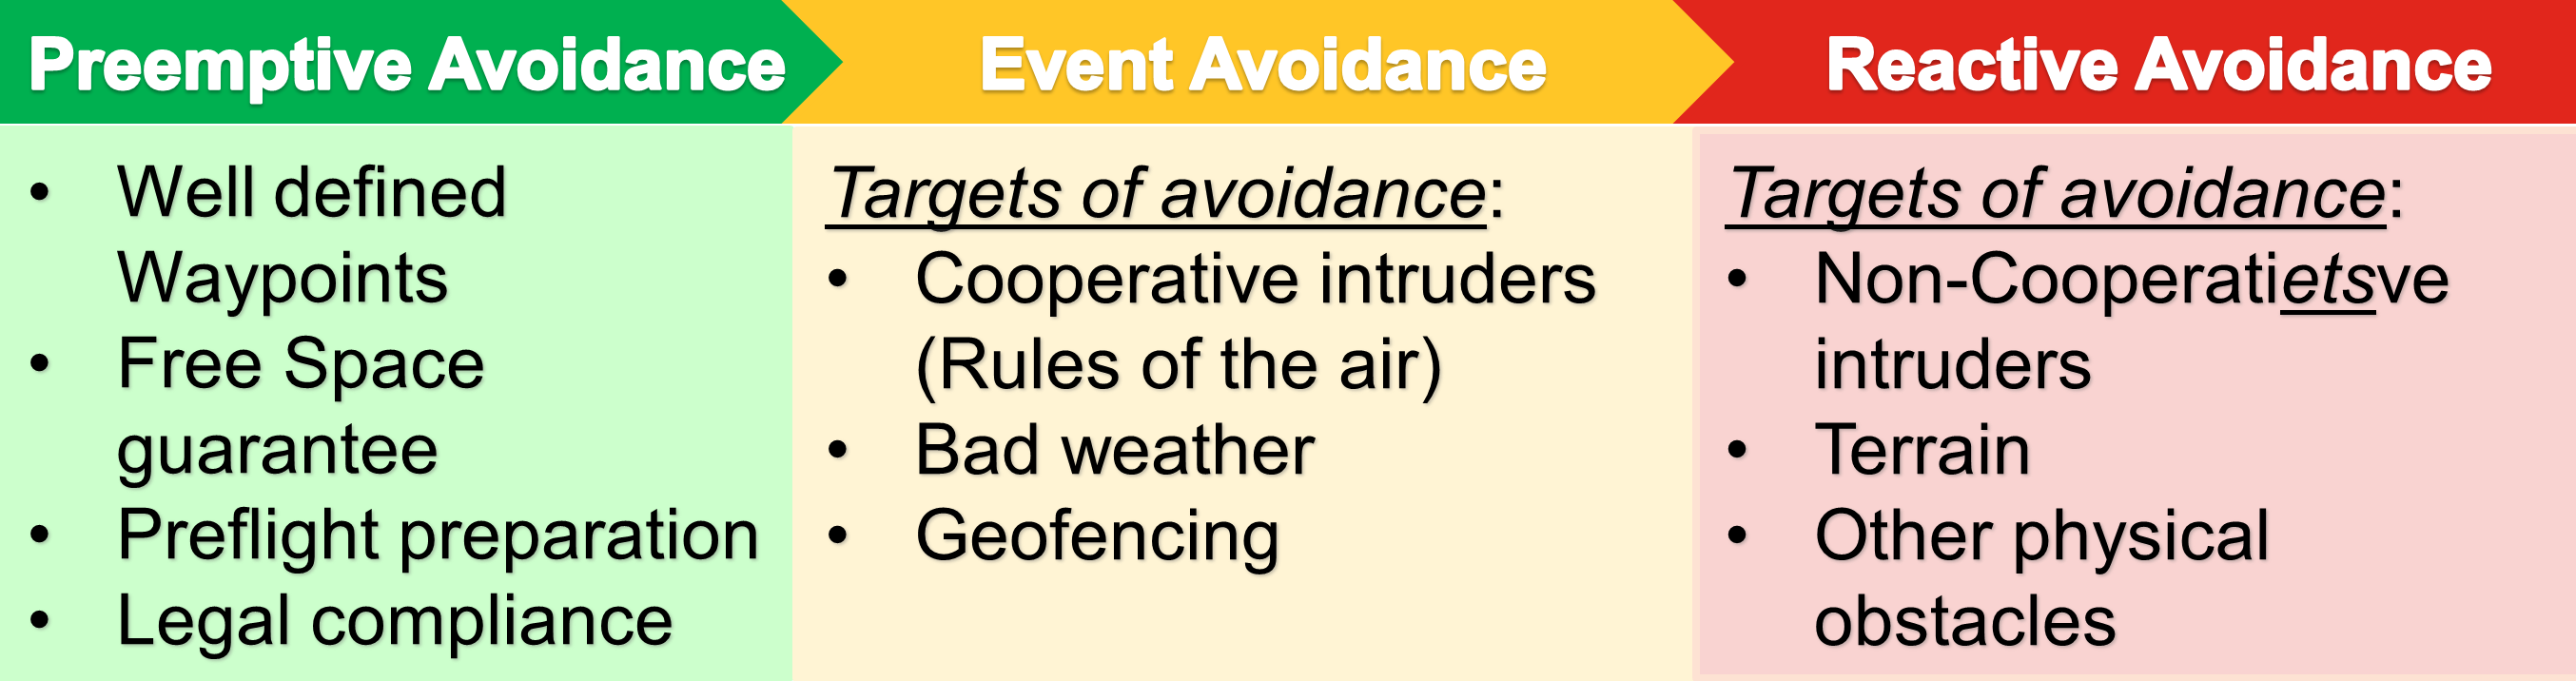
\includegraphics[width=0.7\linewidth]{\FIGDIR/RE001AvoidanceLevelsBasedOnReactionTime} 
    \caption{Avoidance levels based on reaction time.}
    \label{fig:AvoidanceLevels}
\end{figure}

\noindent This work will focus on handling \emph{Event Avoidance}, and \emph{Reactive Avoidance} and the \emph{Avoidance Path} will be calculated using \emph{Reach set Based Methods}. 

The \emph{Preemptive Avoidance} is trying to remove any possible threat before the flight. The risk mitigation is tedious and its done only when necessary. Even the best \emph{preemptive} avoidance could fail.

\emph{Reactive Avoidance} is solving most urgent situations with very short reaction opportunity. This work focus on physical obstacles and terrain. Non-cooperative intruders are partially considered. The adversary behavior was is not considered.

\emph{Event Avoidance} has more opportunity to react. Some threats are known prior the flight (geo-fenced areas, etc.). The future UTM implementation is also considered as \emph{Event Avoidance}, due to the time horizon and authority enforcement. 

\paragraph{Basic Idea:} Create deterministic finite-time \emph{Reactive Avoidance} based on \emph{Reach sets} to ensure \emph{trajectory feasibility}. Enhance method with a set of the rules to enable handling more complex situations.

The \emph{Discretization} is the key to ensure calculation in finite time. Finite \emph{partition} of \emph{operational space (Known World)} and finite representation of \emph{Reach set} guarantees finite count of calculation steps. Aircraft conflict prediction mentioned in \cite{prandini2008application}.

\newpage    
\section{Overview}\label{s:approachOverview}

\noindent The \emph{Overview} is based on \emph{Existing} Emergency avoidance framework \cite{gomola2017obstacle} (fig. \ref{fig:avoidanceConcept}). To achieve goals defined in \emph{Problem Definition} (sec. \ref{s:BasicProblemDefinition}, \ref{s:IncrementalProblemDefinition}) following \emph{Avoidance Framework Concept} (fig. \ref{fig:AvoidanceFrameworkConceptNew}) is proposed:

\begin{figure}[H]
    \centering
    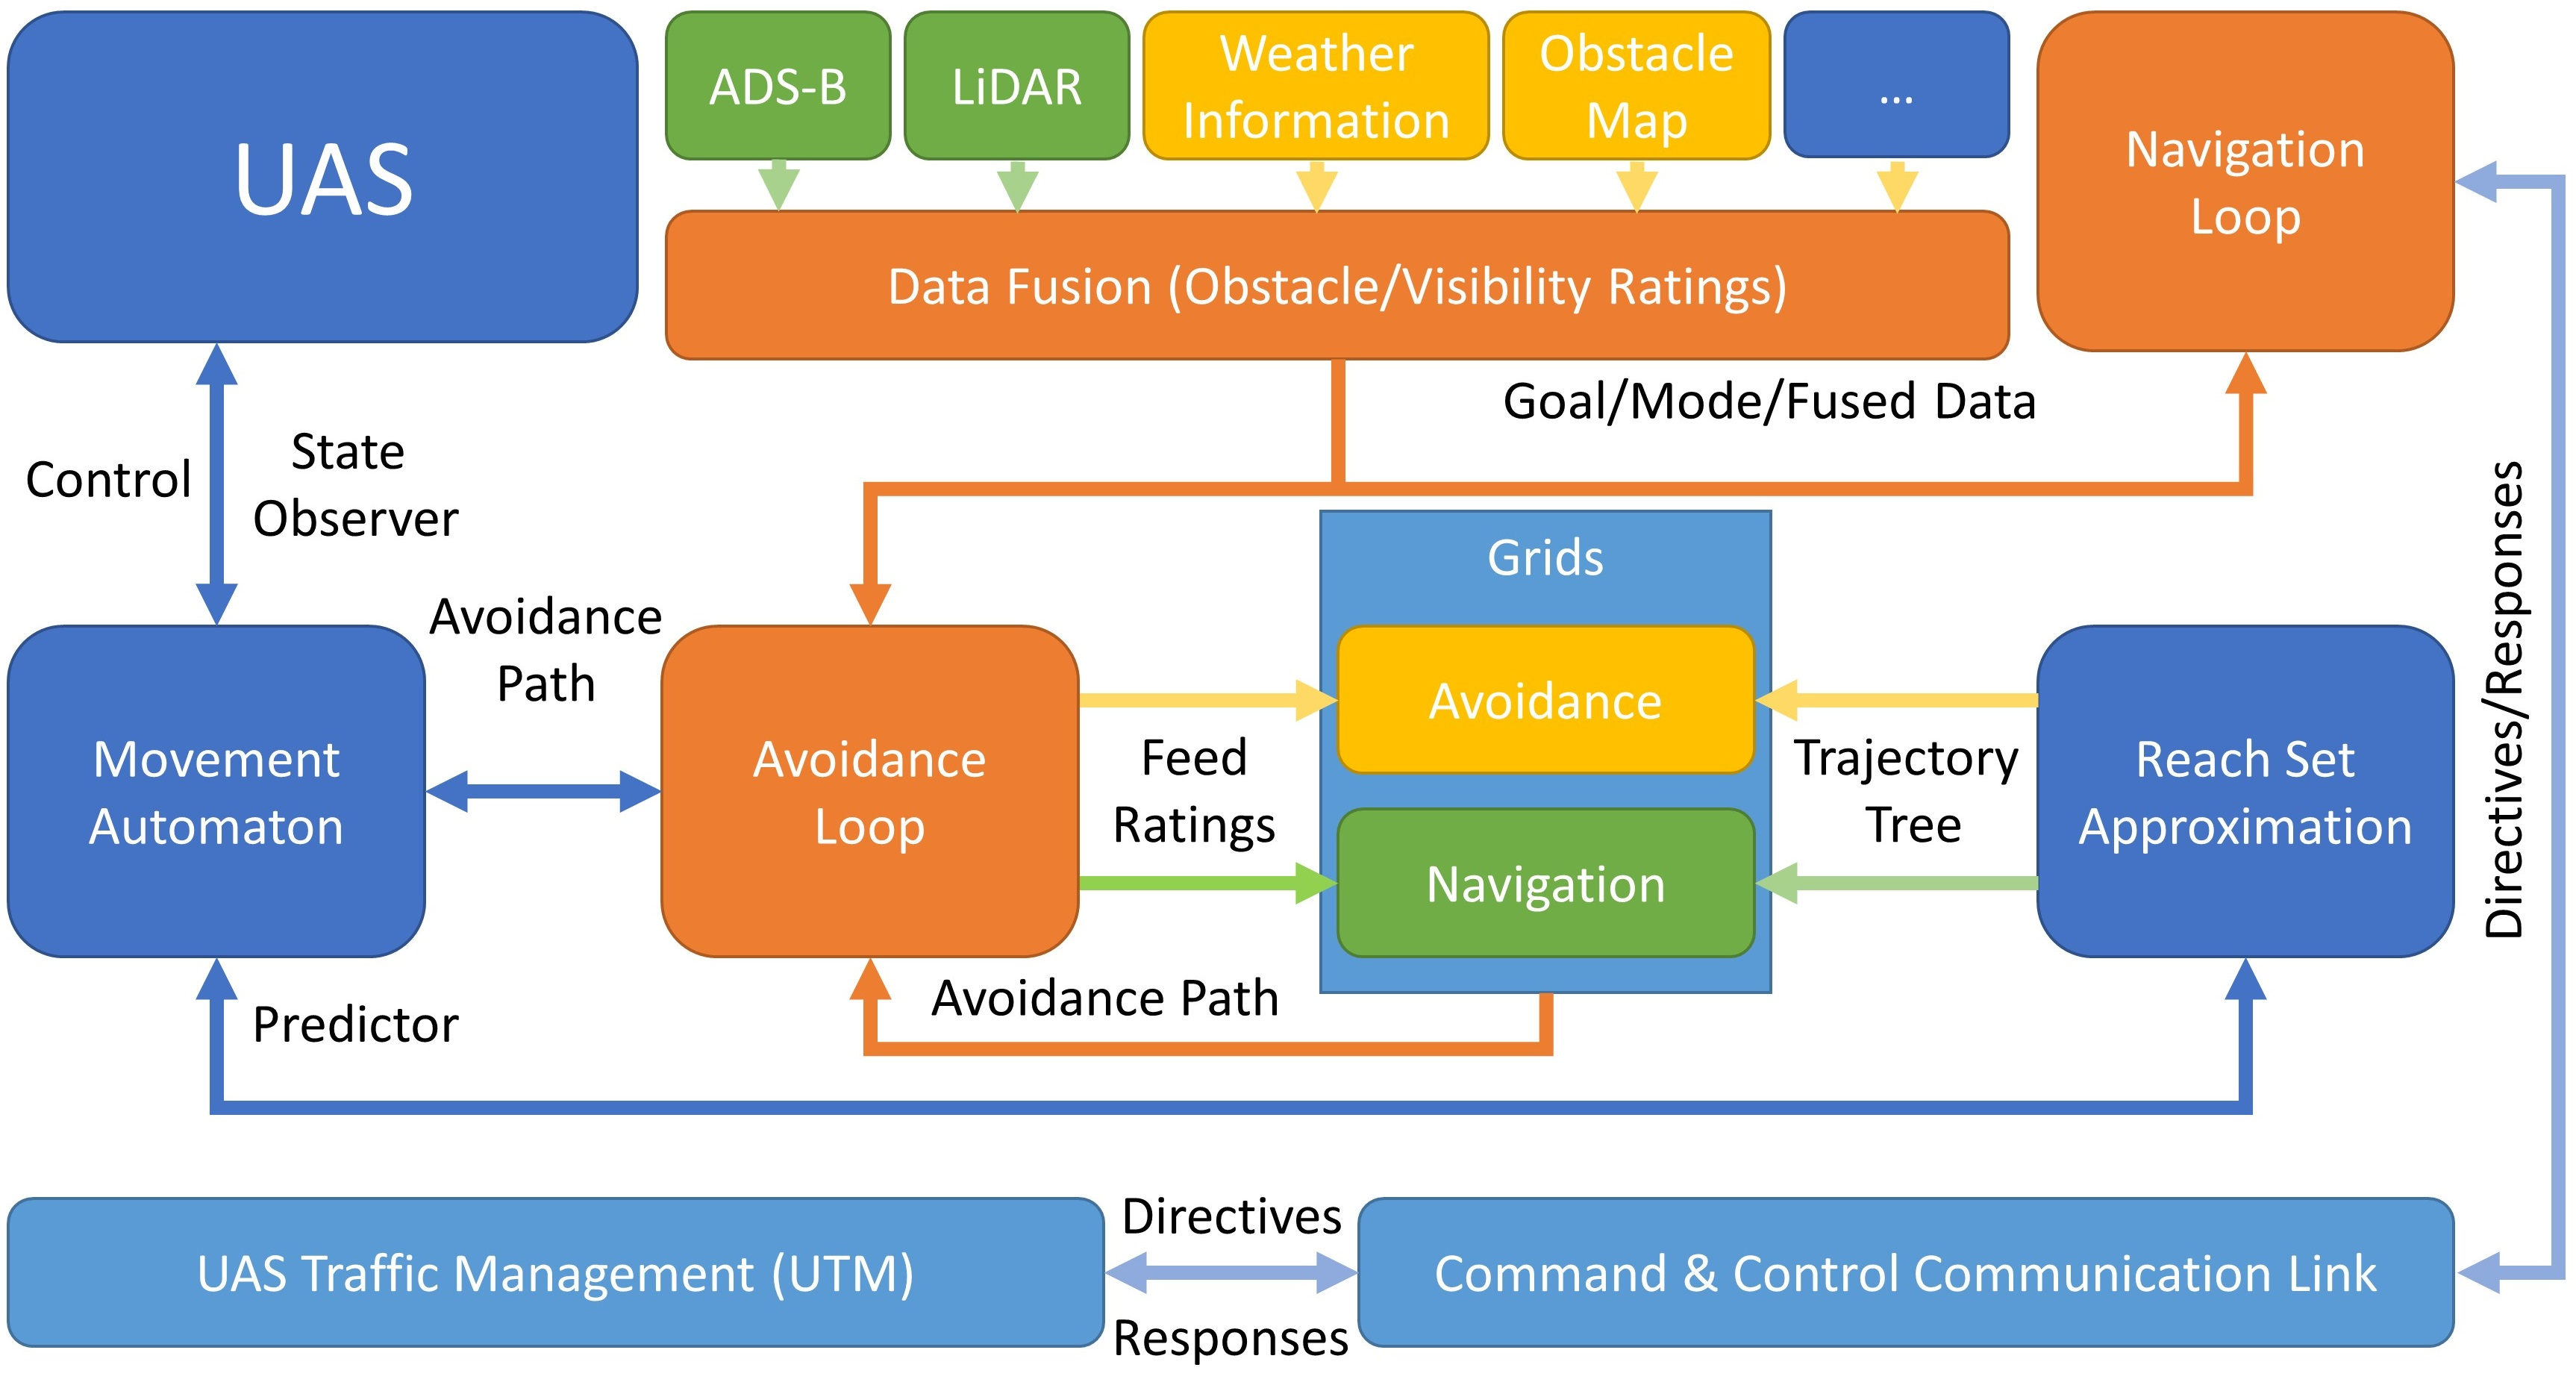
\includegraphics[width=0.95\linewidth]{\FIGDIR/TE037ConceptualSchemeNew} 
    \caption{Avoidance Framework Concept.}
    \label{fig:AvoidanceFrameworkConceptNew}
\end{figure}


\paragraph{Structure of Avoidance Framework:}

\begin{enumerate}
    \item \emph{Unmanned Aircraft System} (UAS) (Role: Controlled Plant) - the \emph{UAS} is controlled via \emph{interface} implemented as \emph{Movement Automaton}. The model used is described in (sec. \ref{s:UASNonlinearModel}).
    
    \item \emph{Movement Automaton} (Role: Control Interface/Predictor) - consumes \emph{Discrete Command Chain} to generate discrete \emph{reference trajectory}, it can  also be used as a predictor of \emph{future UAS states} (sec. \ref{s:referenceTrajectoryGenerator}). The movement Automaton used in this work is given in (sec. \ref{s:movementAutomatonDefinition}). 
    
    \item \emph{Sensor Field} (Role: Surveillance Providers), the following sensors, were considered in this work:
        \begin{enumerate}[a.]
            \item \emph{LiDAR} (Static obstacle detection) - detection of physical obstacles (eq. \ref{eq:naiveObstacleRate})
            
            \item \emph{ADS-B} (Intruder UAS/Plane detection) - detection of intruders who are broadcasting their position and sometimes heading with plans and additional parameters. The \emph{intersection models} are given in (sec. \ref{s:intruders}, app. \ref{s:linearIntersectionModel}, \ref{s:bodyvolumeIntersection}, \ref{s:uncertaintyIntersection}).
        \end{enumerate}
        
    \item \emph{Information Sources} (Role: Known World Information Enhancers): 
        \begin{enumerate}[a.]
            \item \emph{Obstacle Map} (Static Restriction Source) - imposing static soft/hard constraints on \emph{Known Word}/\emph{Operational Space}. Static constraints are given in (sec. \ref{s:virtualConstraints}).
            
            \item \emph{Weather Information} (Static/Dynamic Restriction Source) - imposing static/mo\-vi\-ng soft/hard constraints on \emph{Known World}/\emph{Operational Space}. Moving constraints are given by (def. \ref{def:movingConstraint}).
            
            \item \emph{Other Airspace Restrictions} - like restricted airspace, geo-fencing, and other future constraint sources, all of them are covered by \emph{Static/Dynamic Constraints} for now.
        \end{enumerate}
    
    \item \emph{Data Fusion} (Role: Sensor Input Interface) - is the unifying interface to asses \emph{Operational State Properties} mainly \emph{Obstacle Rating}, \emph{Visibility}, \emph{Map Obstacle Rating}, \emph{Intruder Rating} for a portion of the space. The partial \emph{ratings} are proposed in related sections. The data fusion procedure with \emph{defuzzification} and final assessment into space sets are outlined in (sec. \ref{s:sensorFusion})  
    
    \item \emph{Reach Set Approximation} (Role: Reachability Estimator) - as \emph{data fusion} is providing the situation assessment, the \emph{Reach set} is providing maneuvering capability assessment. The introduction is given in (sec. \ref{s:reachSet}), the properties are defined in (sec. \ref{s:ReachSetPerformanceCriteria}), the approximation methods with constrained expansion are outlined in (sec. \ref{s:chaoticReachSet}, \ref{s:harmonicReachSet}, \ref{s:combinedReachSet}, \ref{s:acasReachSet}). The reach set estimation is the main contribution of this work.
    
    \item \emph{Grids: Navigation/Avoidance} (Role: Operation Space Segmentation \& Situation Evaluation) - space discretization in polar coordinates grid, different reach sets are used for different grid type, defined in (sec. \ref{s:AvoidanceGrid}).
    
    \item \emph{Avoidance loop} (Role: Short Term Decision Maker) - using data from \emph{Sensor fusion} in \emph{Avoidance/Navigation Grid} trimming \emph{Reachable Space} approximated by \emph{Reach Set} generating feasible \emph{Avoidance Path}. \emph{Avoidance Path} is fed to controlling \emph{Movement Automaton}. The Goal is given by \emph{Navigation Loop}. Avoidance loop is given in (sec. \ref{s:aviudabceGridRun}).
    
    \item \emph{Navigation loop} (Role: Long Term Decision Maker) - using data from \emph{Avoidance Loop}, \emph{Mission plan} and \emph{UTM} directives defines the current long term navigation goal. Details are given in (sec. \ref{s:missionControlRun}).
    
    \item \emph{Command and Control Communication Link} (C2 Link) (Role: Communication Link) - standard communication link with sufficient reliability.
    
    \item \emph{UAS Traffic Management} (UTM) (Controlled Airspace Authority) - checking possible collisions and enforces counter-measurements. Details are given in (sec. \ref{sec:UASTrafficManagement}).
    
\end{enumerate}

\paragraph{Communication in Avoidance Framework:}
\begin{enumerate}
    \item \emph{UAS $\leftrightarrow$ Movement Automaton} - sharing \emph{actual system state}, commanding the UAS platform.
    
    \item \emph{Reach Set $\leftrightarrow$ Movement Automaton} - predicting a set of feasible trajectories for the given situation.
    
    \item \emph{Reach Set $\leftrightarrow$ Grids} - providing trajectory set depending on the active mode (Navigation/Emergency Avoidance).
    
    \item \emph{Avoidance Loop $\leftrightarrow$ Data Fusion} - assessing the situation in \emph{operational space} based on sensor readings/information sources.
    
    \item \emph{Avoidance Loop $\leftrightarrow$ Navigation Loop} - determining long term goal based on situation assessment and UTM directives. 
    
    \item \emph{Avoidance Loop $\to$ Grids} - feeding assessment data and constraints into selected operational space Grid.
    
    \item \emph{Grids $\to$ Avoidance Loop} - returning feasible and \emph{cost-effective} avoidance path after situation assessment and \emph{Reach set} pruning.
    
    \item \emph{Avoidance Loop $\to$ Movement Automaton} - issuing and monitoring movement commands based on actual \emph{avoidance strategy}.
    
    \item \emph{Navigation Loop $\leftrightarrow$ C2 Link $\leftrightarrow$ UTM} - communication to receive directives and send fulfillment. 
\end{enumerate}

   
\end{document}
